\documentclass[12pt,titlepage]{article}

\usepackage{geometry}
\geometry{
    a4paper,
    total={210mm,297mm},
    left=20mm,
    right=20mm,
    top=20mm,
    bottom=20mm,
}

	
\usepackage[]{subcaption}

\usepackage{pdflscape}

% Polski
\usepackage[]{polski} 
\usepackage[polish]{babel}

%do tabel
\usepackage{multirow}

% Pierwszy akapit - wcięty
\usepackage[]{indentfirst}

% Matematyka
\usepackage[]{amsfonts}

\usepackage[]{amsmath}

% Formatowanie
\usepackage{ragged2e}

% Tytuły sekcji
\usepackage{titlesec}
%\titleformat{\section}[block]{\Large\bfseries}{}{1em}{}

% <=
\usepackage{amssymb}

% eps
\usepackage{graphicx}
% \usepackage{subfigure}

% Tabele
\usepackage{array}

\usepackage[style=czech]{csquotes}

\renewcommand*{\thesubsubsection}{}

\usepackage{hyperref}
\hypersetup{
    colorlinks,
    citecolor=black,
    filecolor=black,
    linkcolor=black,
    urlcolor=black
}

\usepackage[numbered]{matlab-prettifier}
\lstset{
    literate={ą}{{\k{a}}}1
    {Ą}{{\k{A}}}1
    {ę}{{\k{e}}}1
    {Ę}{{\k{E}}}1
    {ó}{{\'o}}1
    {Ó}{{\'O}}1
    {ś}{{\'s}}1
    {Ś}{{\'S}}1
    {ł}{{\l{}}}1
    {Ł}{{\L{}}}1
    {ż}{{\.z}}1
    {Ż}{{\.Z}}1
    {ź}{{\'z}}1
    {Ź}{{\'Z}}1
    {ć}{{\'c}}1
    {Ć}{{\'C}}1
    {ń}{{\'n}}1
    {Ń}{{\'N}}1
}

\title{

\includegraphics[scale=0.75]{img/politechnika_sl_logo_bw_poziom_pl.eps}\\
\textbf{Wydział Automatyki, Elektroniki\\
i Informatyki}\\
\vspace*{1cm}
Systemy Interaktywne i Multimedialne \\ Projekt \\ Detekcja emocji w głosie

\vspace*{5cm}
}
\author{
Natalia Stręk
Jakub Kula,
Paweł Wójtowicz,
} 
\date{Gliwice 2023}

\begin{document}

\maketitle

% \tableofcontents

\newpage
\section{Analiza wyników i wnioski}
% Cele i zadania z okresu objętego sprawozdaniem, których realizację już podjęto. Należy odnieść się do zaakceptowanego dokumentu Informacje o realizowanym projekcie (ok 100 słów)\\
Celami wybranymi na okres marzec-kwiecień było napisanie wykonanie odpowiedniego research na temat przetwarzania ludzkiego głosu, oraz parametrów go charakteryzujących. Kolejnym celem było skryptu przetwarzającego dane, wyciagającego opisane charakterystyczne parametry. Ostatnim celem na okres było stworzenie modelu sieci neuronowej posiadajacej minium 50\% dokładności. Jest to model referencyjny do którego będą porónywane kolejne stworzone modele.\\

% Opis zadań przyjętych do realizacji w okresie objętym sprawozdaniem w odniesieniu do poszczególnych etapów pracy. Które z zadań zostały wykonane? Które z zadań są realizowane? Jaki jest procentowy postęp prac? Ile przeznaczono czasu na wykonanie poszczególnych zadań? (ok 300 słów)\\

W trakcie okrsu marzec-kwiecień zostały wybrane cechy dziwięku które zostały użyte jako wejścia do sieci neuronowej.

Wybrane parametry sieci:
\begin{itemize}
    \item \textbf{Chroma STFT}: Reprzentacja częstotliwości dźwięku w sposób związany z tonalnością, używana w analizie akordów i melodii.
    \item \textbf{MFCC}: Kompaktowa reprezentacja dźwięku, oparta na skali melowej, często stosowana w rozpoznawaniu mowy i dźwięku.
    \item \textbf{Root Mean Square Value}: Średnia wartość kwadratu sygnału dźwiękowego, stosowana do oceny głośności.
    \item \textbf{Spectral Centroid}: Średnia częstotliwość w spektrum dźwięku, służy do oceny barwy dźwięku.
    \item \textbf{Spectral Spread}: Mierzona rozpiętość częstotliwości w spektrum dźwięku, informuje o jego różnorodności częstotliwości.
    \item \textbf{Spectral Flux}: Miara zmienności spektrum dźwięku w czasie, używana w analizie dynamiki dźwięku.
    \item \textbf{Spectral Roll-Off}: Częstotliwość, poniżej której kumulatywna energia spektrum jest mniejsza niż określony procent całkowitej energii.
    \item \textbf{Chroma Vector}: Wektor reprezentujący rozkład mocy dźwięku w chromie, używany w analizie harmonicznej.
    \item \textbf{MelSpectrogram}: Spektrogram dźwięku, gdzie skala częstotliwości jest przekształcona na skalę melową, co odzwierciedla sposób, w jaki ludzkie ucho percepcyjnie odbiera dźwięki.
\end{itemize}

W celu zmniejszenia wymiarowości/ilości wejść do sieci, została wyciągnięta średnia z każdego parametru z każdego segmentu czasowego.\\

Została także wytrenowana sieć podstawowa. Sieć tak osiąga 68\% dokładności na zbiorze uczącym oraz 45\% na zbiorze testującym.\\
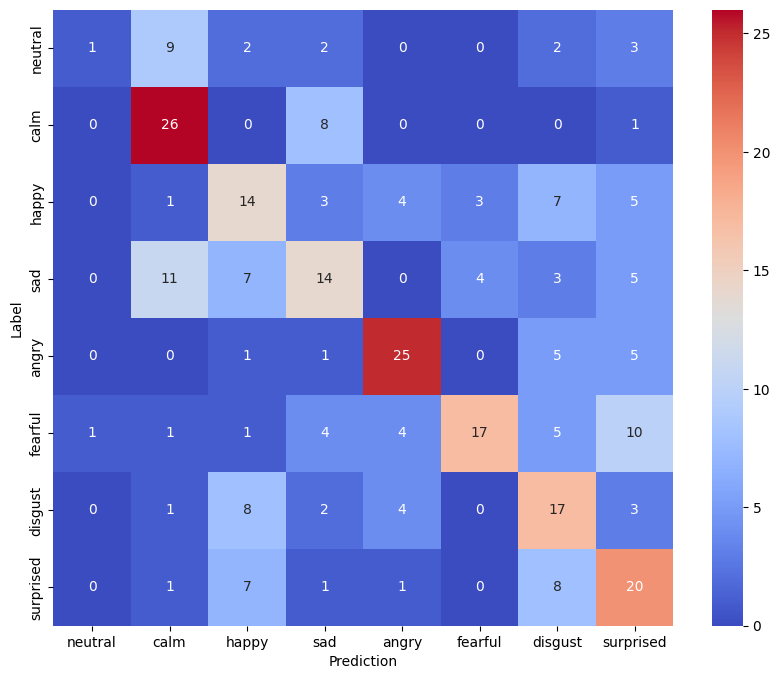
\includegraphics[width=\linewidth]{img/error_matrix.png}

% Czy projekt realizowany jest zgodnie z harmonogramem? Jeśli nie, podać przyczyny opóźnień w odniesieniu do etapów pracy oraz opisać działania naprawcze mających na celu osiągnięcie celów i wyników projektu\\
Projekt jest realizowany zgodnie z harmonogramem.\\

% Czy wprowadzono jakieś znaczące zmiany do zrealizowanych działań lub w składzie zespołu? Jeśli tak, opisać jakie oraz podać ich wpływ na realizację projektu.
Wprowadzono następujące zmiany w założeniach projektu:
Dodano kolejny zbiór nagrań. Zbiór TESS  Toronto emotional speech set posiada aż 2800 nagrań podzielonych na 6 klas.  Do projektu użytko tylko nagrań audio. Klasy to: neutral, happy, sad, angry, fearful, surprise i disgust. Zbiór TESS nie posiada emocji calm który posiadał zbiór Ravdess.\\
Kolejną zmianą jest zmniejszenie długości nagrań głosowych do jednej sekundy. Zostało to zastosowane ze względu na to, że wszystkie nagrania muszą mieć taką samą długość, a dane z nowego zbioru są znacząco krótsze. Dane ze zbioru Ravdess zostały użyte od 0.6s do 1.6s.

\end{document}